\documentclass[a4paper, 12pt]{article}

\usepackage{cmap}
\usepackage{mathtext} 
\usepackage[T2A]{fontenc}
\usepackage[utf8]{inputenc}
\usepackage[english,russian]{babel}	

\usepackage{amsfonts,amssymb,amsthm,mathtools}
\usepackage{amsmath}
\usepackage{icomma} 

\usepackage{graphicx} 
\graphicspath{{Picturies/}}
\usepackage{wrapfig}

\usepackage{array,tabularx,tabulary,booktabs}
\usepackage{longtable}
\usepackage{multirow}

\usepackage{caption}
\captionsetup{labelsep=period}

\renewcommand{\phi}{\varphi}
\newcommand{\eps}{\varepsilon}
\renewcommand{\AA}{\ensuremath{\mathring{A}}}
\newcommand{\parag}[1]{\paragraph*{#1:}}

\newcounter{Points}
\setcounter{Points}{1}
\newcommand{\point}{\arabic{Points}. \addtocounter{Points}{1}}

\author{Вязовцев Андрей, Б01-005}
\date{20.09.22}
\title{Лабораторная работа 5.2.2 - 5.2.3. Изучение спектров атома водорода и молекулы йода.}

\begin {document}

\maketitle

\parag {Цель работы} Изучить сериальные закономерности в оптическом спектре водорода и спектр поглощения паров йода в видимой области.

\parag {В работе используются} установка для проведения опыта, водородная лампа, ртутная лампа, неоновая лампа, лампа накаливания и камера с парами йода.

\parag {Теоретическая справка} ~\\

Атом водорода является простейшей атомной системой, поэтому спектр атома водорода --- предмет тщательного исследования. Длины волн спектральных линий водородноподного атома описываются формулой:

\begin{equation}
    \frac{1}{\lambda_{mn}} = R Z^2 \left( \frac{1}{n^2} - \frac{1}{m^2} \right)
    \label {eq:gen_spec}
\end{equation}

где $R = 109677.6 ~ см^{-1}$ --- постоянная Ридберга, а $m$ и $n$ --- целые числа.

Для объяснения этого явления стоит рассмотреть постулаты Бора:

\begin{enumerate}
    \item В атоме осуществляются только некоторые стационарные орбиты, при движении по которым электрон не излучает энергии.
    \item Из всех орбит реализуются только те, для которых момент количества движения кратен постоянной Планка.
    \item Излучение или поглощение происходит при переходе между стационарными состояниями, при этом:
    \[
        h\nu = E_2 - E_1
    \]
\end{enumerate}

В случае молекул всё сложнее: они обладают более богатым спектром возбуждённых состояний. В первом приближении их волновую функцию можно разбить на три независимых: соответствующию электронным движениям, колебаниям и вращениям молекулы.

\[
    \psi = \psi_{эл} \cdot \psi_{колеб} \cdot \psi_{вращ}
\]

При смещении атомов в молекуле из равновесных положений могут возникать колебания около положения равновесия. В результате действия различных сил образуется потенциальный минимум. Энергия колебаний квантуется:

\[
    E_{колеб} = \hbar \omega_0 \left(n + \frac{1}{2}\right) - \hbar \omega x_n \left(n + \frac{1}{2} \right)^2 \approx \hbar \omega_0 \left(n + \frac{1}{2}\right)
\]

где $x_n$ --- коэффициент анахронизма, который, обычно, мал, а $n$ --- колебательное квантовое число.

Энергия вращения тоже квантуется:

\[
    E_{вращ} = \frac{\hbar^2}{2J} l (l+1), ~ l = 0,1, \cdots
\]

Теперь рассмотрим оптические переходы в молекулах. С ростом $n$ растёт амплитуда колебаний. При достижении некоторой максимальной амплитуды происходит разрыв связи между атомами, т.~е. диссоциация молекулы. Наименьшая энергия, чтобы произошло такое --- энергия диссоциации.

\parag {Экспериментальная установка} ~

На рис. \ref{img:work1} изображена схема установки. На ней:

\begin{itemize}
    \item 1 --- входная щель.
    \item 2 --- коллиматорный объектив.
    \item 3 --- сложная спектральная призма, склеенная из $П_1$, $П_2$ и $П_3$.
    \item 4 --- объектив зрительной трубы.
    \item 5 --- окуляр зрительной трубы.
    \item 6 --- поворотный столик для 3.
    \item 7 --- микрометрический винт с отсчётным барабаном для 6.
    \item 8 --- микрометрический винт для 2.
    \item 9 --- микрометрический винт для 1.
    \item 10 --- острие указателя.
    \item 11 --- массивный корпус, спасающий установку от студентов.
    \item Л --- источник света.
    \item К --- конденсор (для концентрации света на входной щели).
    \item Оптическая скамья --- нужна для размещения Л и К.
    \item Пульт управления.
\end{itemize}

\begin{figure}[!h]
    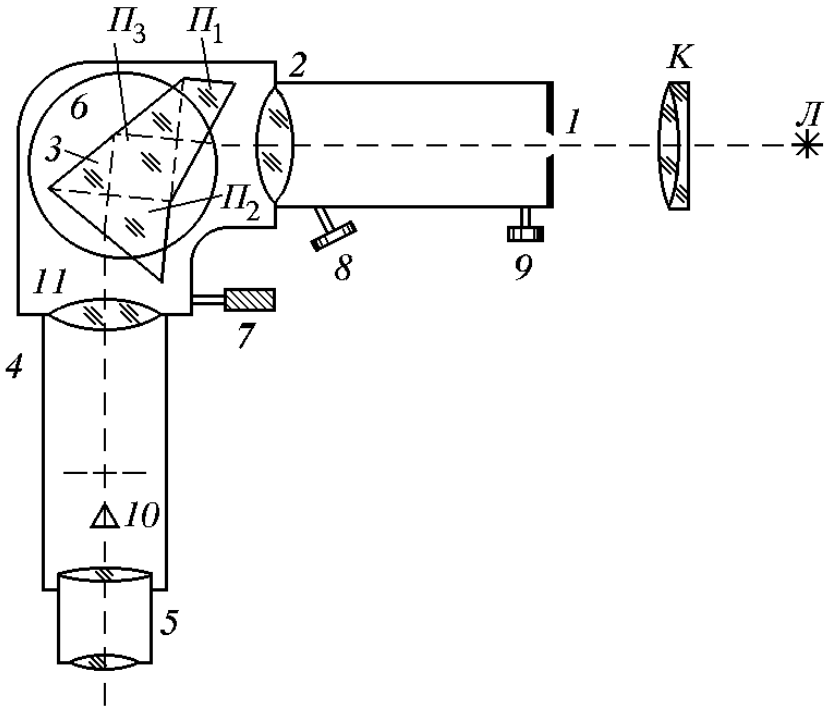
\includegraphics[scale = 0.4]{Workplace1}
    \centering
    \caption{Схема экспериментальной установки}
    \label{img:work1}
\end{figure}

В случае с йодом схема немножко усложняется, т.~к. вместо лампы с конкретным веществом будет использоваться источник белого света (лампа накаливания) (1), которая светит на кювету с йодом (2). Приблизительная схема установки изображение на рис. \ref{img:work2}.

\begin{figure}[!h]
    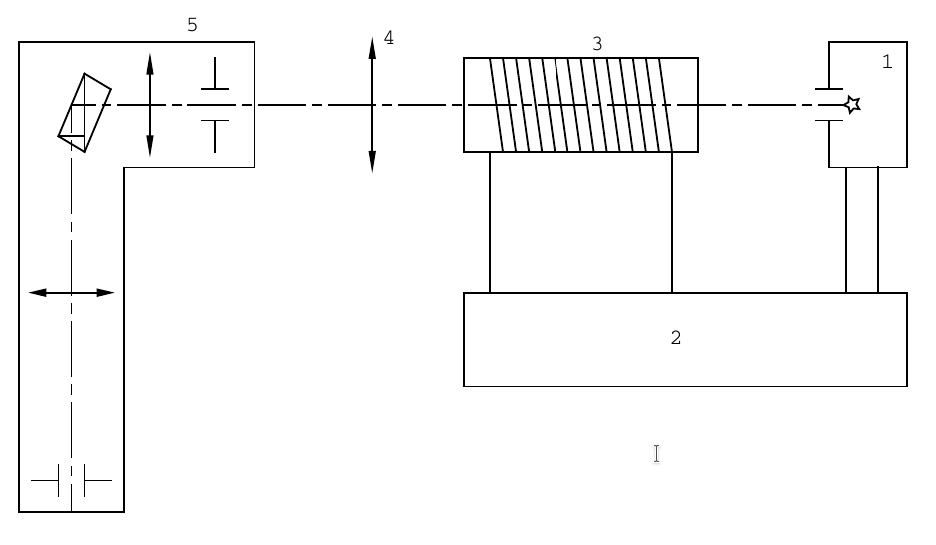
\includegraphics[scale = 0.4]{Workplace2}
    \centering
    \caption{Схема экспериментальной установки}
    \label{img:work2}
\end{figure}

\parag {Ход работы} ~\\

\point Ознакомимся с принципом работы установки. Включим её и неоновую лампу в сеть, отцентруем её по высоте. Конденсор расположим в 25 см от щели. Настроимся на резкое изображение кончика указателя, вращая глазную линзу окуляра. Отрегулируем яркость освещения указателя с помощью реостата.

\point Вращая барабан, настроимся на жёлтую линию неона (она одна из самых ярких). Перемещая коллиматор винтом 8, получим резкое изображение.

\point Найдём нуль микрометрического винта, для этого будем всё медленнее и медленнее открывать щель с помощью винта 9, фиксируя момент появления света. Получаем:

\begin{table}[!h]
    \centering
    \begin{tabular}{|c|c|c|c|}
        \hline
        № & 1 & 2 & 3\\ \hline
        $l$, 10 мкм & 20 & 19 & 17 \\ \hline
    \end{tabular}
    \caption {Настройка щели винта.}
\end{table}

Итак, 170 мкм --- ноль винта. Откроем щель на $0.05$ мм, т.~е. поставим винт 9 на значение 220 мкм.

\point Закончим насторйку окуляра. Для этого сделаем резкость такой, чтобы параллакс (т.~е. смещение указателя относительно линии при движении глаза) отсутствовал.

\point Теперь проведём градуировку спектрометра по спектрам неона и ртути. Для этого запишем расположение их спектральных линий на барабане и соответствующие им табличные значения длин волн. Результаты представлены в таблицах \ref{tab:neon} и \ref{tab:hydr}.

\begin{table}[!h]
    \centering
    \begin{tabular}{|c|c|c|c|c|c|c|c|c|c|}
        \hline
        n & 1 & 2 & 3 & 4 & 5 & 6 & 7 & 8 & 9 \\ \hline
        $\lambda$, $\AA$ & 7032 & 6929 & 6717 & 6678 & 6599 & 6533 & 6507 & 6402 & 6383 \\ \hline
        $\phi$, $~^\circ$ & 2914 & 2888 & 2822 & 2808 & 2778 & 2758 & 2748 & 2712 & 2704 \\ \hline
    \end{tabular}
    \\~\\
    \begin{tabular}{|c|c|c|c|c|c|c|c|c|}
        \hline
        n & 10 & 11 & 12 & 13 & 14 & 15 & 16 & 17 \\ \hline
        $\lambda$, $\AA$ & 6334 & 6305 & 6267 & 6217 & 6164 & 6143 & 6096 & 6074 \\ \hline
        $\phi$, $~^\circ$ & 2686 & 2674 & 2660 & 2640 & 2618 & 2608 & 2590 & 2578 \\ \hline
    \end{tabular}
    \\~\\
    \begin{tabular}{|c|c|c|c|c|c|c|c|c|}
        \hline
        n & 18 & 19 & 20 & 21 & 22 & 23 & 24 & 25 \\ \hline
        $\lambda$, $\AA$ & 6030 & 5976 & 5945 & 5882 & 5852 & 5401 & 5341 & 5331 \\ \hline
        $\phi$, $~^\circ$ & 2558 & 2534 & 2518 & 2490 & 2474 & 2212 & 2172 & 2168
        \\ \hline
    \end{tabular}
    \caption {Спектр неона.}
    \label{tab:neon}
\end{table}

\begin{table}[!h]
    \centering
    \begin{tabular}{|c|c|c|c|c|c|c|c|c|c|}
        \hline
        n & K1 & K2 & 1 & 2 & 3 & 4 & 5 & 6\\ \hline
        $\lambda$, $\AA$ & 6907 & 6234 & 5791 & 5770 & 5461 & 4916 & 4358 & 4047\\ \hline
        $\phi$, $~^\circ$ & 2880 & 2648 & 2444 & 2440 & 2250 & 1830 & 1164 & 614
        \\ \hline
    \end{tabular}
    \caption {Спектр ртути.}
    \label{tab:hydr}
\end{table}

\point Перейдём к измерению линий спектра водорода. Результаты можно увидеть в таблице \ref{tab:gen}.

\begin{table}[!h]
    \centering
    \begin{tabular}{|c|c|c|c|c|}
        \hline
        n & $H_\alpha$ & $H_\beta$ & $H_\gamma$ & $H_\delta$ \\ \hline
        $\phi$, $~^\circ$ & 2768 & 1780 & 1136 & 718 \\ \hline
    \end{tabular}
    \caption {Спектр водорода.}
    \label{tab:gen}
\end{table}

\point Далее исследуем спектр йода. Т.~к. установка слегка изменилась, произведём центровку заново. Сделаем три измерения, результаты находятся в таблице \ref{tab:iod}:

\begin{enumerate}
    \item Самая длинноволновая хорошо видимая линия поглощения ($n_{1.0}$).
    \item Шестая по счёту линия от выбранной ранее ($n_{1.5}$).
    \item Граница схождения спектра, т.~е. начало сплошного спектра поглощения ($n_{гр}$).
\end{enumerate}

\begin{table}[!h]
    \centering
    \begin{tabular}{|c|c|c|c|}
        \hline
        n & $n_{1.0}$ & $n_{1.5}$ & $n_{гр}$ \\ \hline
        $\phi$, $~^\circ$ & 2630 & 2532 & 1960 \\ \hline
    \end{tabular}
    \caption {Спектр йода.}
    \label{tab:iod}
\end{table}

\parag {Обработка результатов} ~\\

\point Составим градуировочную кривую с помощью линий спектра неона и ртути. Исходя из предположения, что эта кривая задаётся формулой вида:

\[
    \lambda = a e^{b \phi} + c
\]

Найдём коэффициенты $a$, $b$ и $c$ с помощью МНК. Результаты представлены на рис. \ref {img:calib}:

\begin{figure}[!h]
    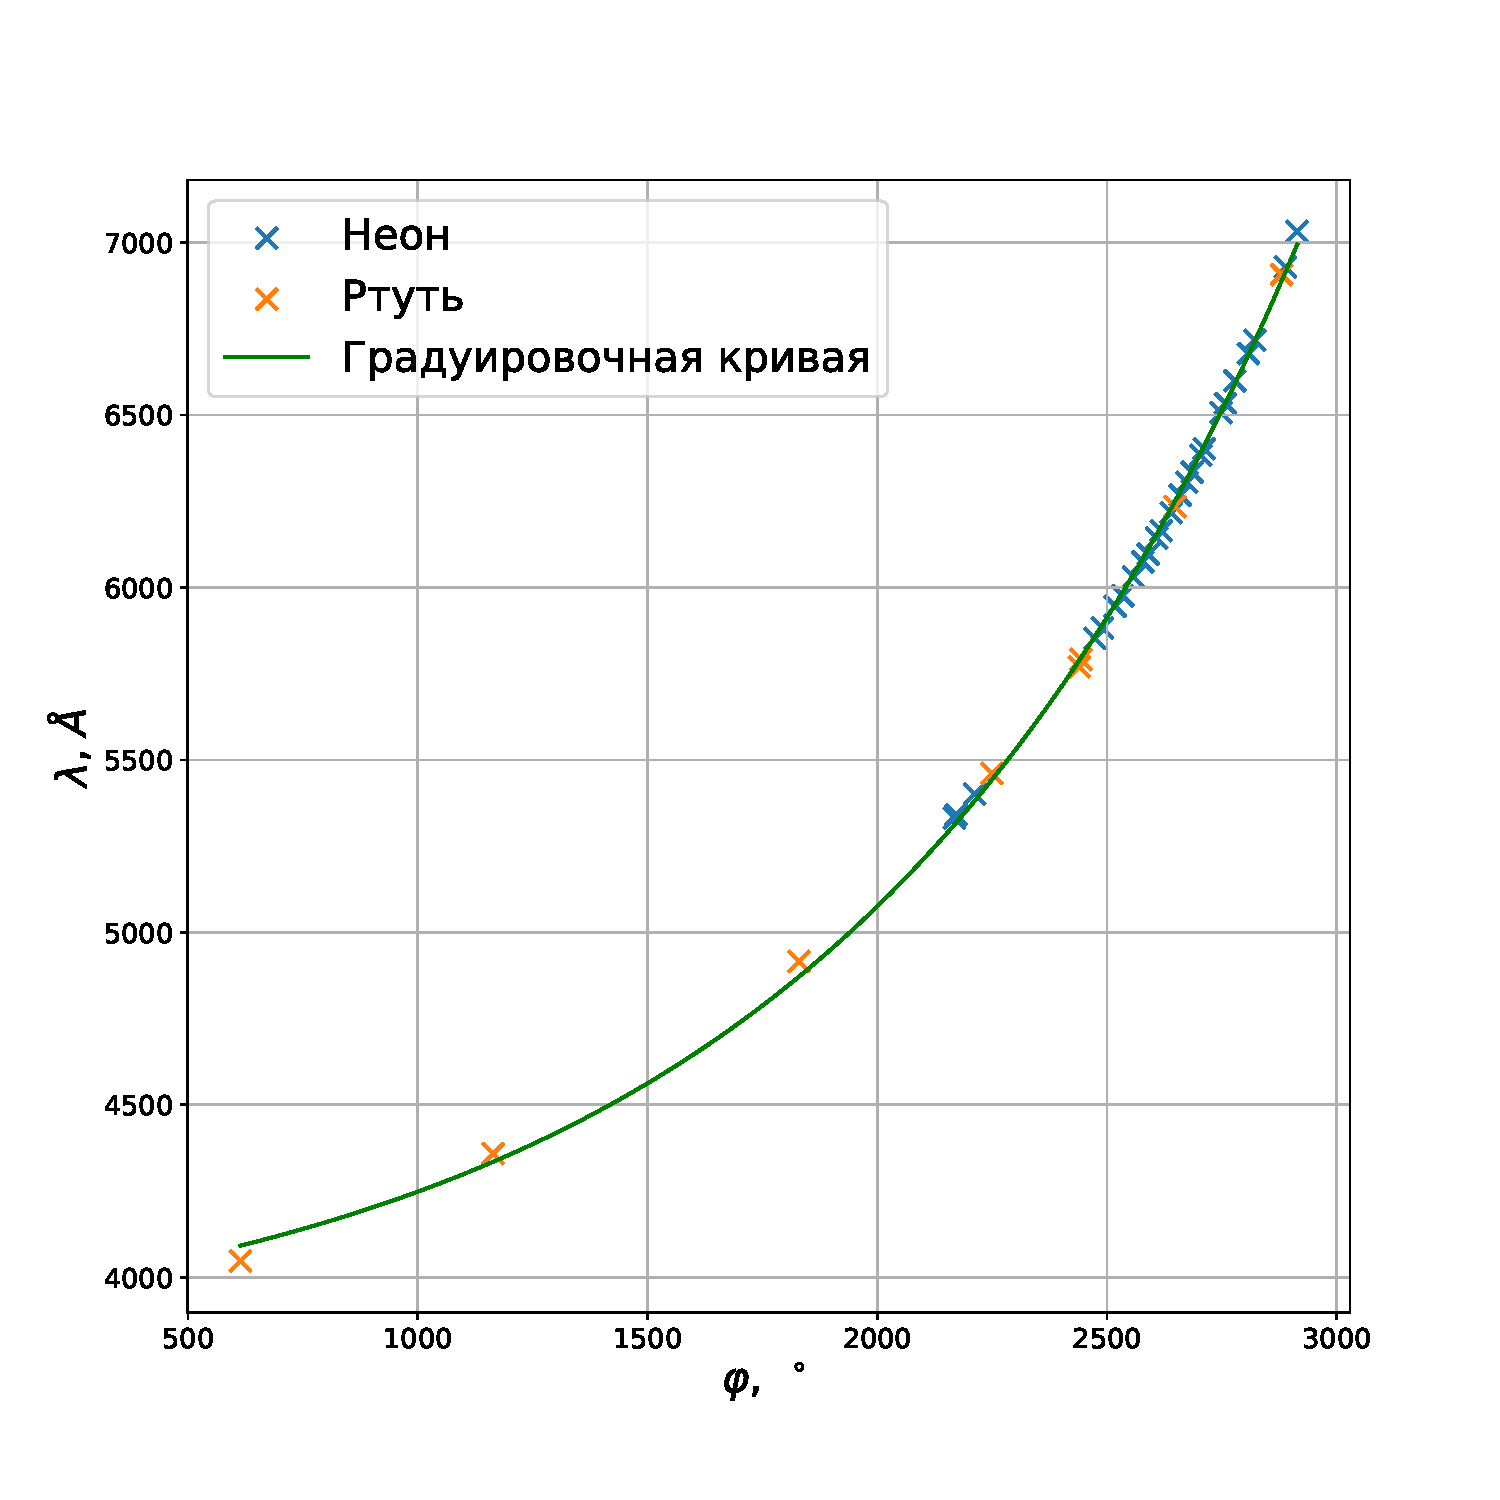
\includegraphics[scale = 0.35]{calib}
    \centering
    \caption{Калибровочный график}
    \label{img:calib}
\end{figure}

\begin{align*}
    a &= (186 \pm 10) \AA \\
    b &= (9.80 \pm 0.16) \cdot 10^{-4} \AA \\
    c &= (3750 \pm 30) \AA \\
\end{align*}

\point С помощью этой кривой определим длины волн линий водорода:

\begin{align*}
    \lambda_\alpha &= (6560 \pm 300) ~ \AA \\
    \lambda_\beta  &= (4810 \pm 120) ~ \AA \\
    \lambda_\gamma &= (4310 \pm 70)  ~~ \AA \\
    \lambda_\delta &= (4120 \pm 50)  ~~ \AA
\end{align*}

Это довольно совпадает в рамках погрешности с табличными значениями: $\lambda_\alpha = 6562.8 ~ \AA$, $\lambda_\beta = 4861.4 ~ \AA$, $\lambda_\gamma = 4340.5 ~ \AA$, $\lambda_\delta = 4101.7 ~ \AA$.

\point Найдём постоянную Ридберга для каждого случая по формуле \eqref{eq:gen_spec}.

\begin{align*}
    R_\alpha &= (110000 \pm 5000) ~ см^{-1} \\
    R_\beta  &= (111000 \pm 3000) ~ см^{-1} \\
    R_\gamma &= (110300 \pm 1800) ~ см^{-1} \\
    R_\delta &= (109000 \pm 1400) ~ см^{-1}
\end{align*}

Учитывая, что $R = 109677.6 ~ см^{-1}$, можно сказать, что константа найдена верно в рамках погрешности.

\point Определим, аналогично предыдущим пунктам, длины волн для измерений у йода:

\begin{align*}
    \lambda_{1.0} &= 6200 \pm 300 \\
    \lambda_{1.5} &= 6000 \pm 300 \\
    \lambda_{гр}  &= 5020 \pm 140
\end{align*}

\point Вычислим энергию колебательного кванта в электронвольтах:

\[
    h\nu_2 = \frac{h\nu_{1.5} - h\nu_{1.0}}{5} = (15.0 \pm 1.7) \cdot 10^{-3} ~ эВ
\]

\point Из информации, что $h\nu_1 = 0.027$ эВ (энегрия колебательного кванта основного состояния), $E_A = 0.94$ эВ (энергия возбуждения атома), вычислим:

\begin{enumerate}
    \item Энергию электронного перехода $h\nu_{эл}$:
    \[
        h\nu_{эл} = h\nu_{1.0} - \frac{1}{2} \cdot h\nu_2 + \frac{3}{2} \cdot h\nu_{1} = (2.04 \pm 0.10) ~ эВ
    \]
    \item Энергию диссоциации молекулы в основном состоянии $Д_1$:
    \[
        Д_1 = h\nu_{гр} - Е_A = (1.53 \pm 0.10) ~ эВ
    \]
    \item Энергию диссоциации молекулы в возбуждённом состоянии $Д_2$:
    \[
        Д_2 = h\nu_{гр} - h\nu_{эл} = (0.43 \pm 0.10) ~ эВ
    \]
\end{enumerate}

\end {document}
